\chapter{Ausblick}\label{ch:ausblick}
Je weiter sich das Projekt der vorliegenden Arbeit dem Abschluss näherte desto mehr kristallisierte sich ein Hauptproblem heraus.
Das erstellte Template ist sehr auf die DATEV Rechnungsschreibung spezialisiert, das heißt, es ist funktionsfähig, kann aber nicht ohne zeitaufwändige Eingriffe in das Template, in die Workflowdefinitionsdateien und die eigentlichen REXX Skripte und Jobs, an eine andere Anwendung angepasst werden. 
Zusätzlich ist der durch den momentanen Stand des Templates ermöglichte Bereitstellungsprozess nicht optimal.
Bei der Betrachtung des Falles, wenn zwei Anwender jeweils eine eigene Instanz des gleichen Templates benötigen, muss dieses kopiert werden und neu in z/OSMF aufgenommen werden.
Dies verlangt Wissen (Kommentar: bei wem)  über die z/OSMF Oberfläche und den Speicherort des Templates, um es schließlich auch ändern zu können.
AUs MQ Sicht ist vor allem kritisch, dass die Bereitstellung eines IBM Queue Managers nicht im Template enthalten ist.
So müsste ein neuer IBM Queue Manager weiterhin manuell angelegt werden und der gewünschte Effekt (weitgehende Automatisierung und Unabhängigkeit von der Administration) schwächt sich ab.
Eine Herangehensweise an dieses Problem wird im Folgenden beschrieben.
Diese ist als Ausblick zu verstehen, die Umsetzung ist kein Bestandteil dieser Arbeit.

Angenommen, das Template beinhaltet die Provisionierung eines IBM Queue Managers, so könnte jeder Entwickler seine eigene Instanz des Templates besitzen und beispielsweise für eigene Tests nutzen.
Da die Application Id einer CICS-Instanz eindeutig sein muss, müsste dennoch jeder Entwickler ein eigenes Template dahingehend anpassen, dass dies gewährleistet ist.
Eine Möglichkeit wäre, einen Pool mit verfügbaren Application IDs bereitzustellen und dann mittels eines Programms eine ungenutzte Application ID zu bestimmen.
Dieses Programm kann dann als Step in das Template aufgenommen werden und das Problem der eindeutigen Application ID wäre gelöst.
Jedoch müsste immer noch für jede kleine Änderung an der Konfiguration des Templates ein neues Template erzeugt werden.
Hier schafft z/OSPT Abhilfe.
Damit kann, wie in Absatz \ref{sssec:zospt} beschrieben, mit Hilfe einer Konfigurationsdatei das Template von außen gesteuert werden.
Dadurch fällt das Kopieren des Template für den Mitarbeiter weg, dieser muss mittels des Kommandozeileninterfaces ein Image bauen und daraus einen Container erzeugen.
Das Kommandozeileninterface hat einen weiteren Vorteil.
Mit dessen Hilfe können Arbeitsschritte für die Provisionierung der Middleware in einen Jenkins-Ablauf aufgenommen werden.
Somit läuft der Prozess automatisiert ab und nähert sich modernen Entwicklungsabläufen wie denen aus der Cloud Native Entwicklung an.

Die Arbeitsweise und der Bereitstellungsprozess für die Laufzeitumgebung, die der DATEV Rechnungsschreibungs-Ablauf benötigt, ist dadurch vereinfacht und es werden weniger Absprachen benötigt.
Allerdings ist das Template weit von einer Nutzung außerhalb der DATEV Rechnungsschreibung entfernt. (Kommentar: jetzt doch wieder TemplateÛ) 
Während der Realisierung dieser Arbeit wurde klar, dass anwendungsspezifische Templates nicht optimal sind und nicht den vollständigen Funktionsumfang von `IBM Cloud Provisioning and Management for z/OS` ausreizen.
So ist zu empfehlen, dass für jedes Subsystem, also CICS, Db2 und IBM MQ, ein separates Template realisiert wird.
Dafür müsste das Template dynamischer implementiert sein.
Um dies zu verdeutlichen, wird als Beispiel die Provisionierung von IBM MQ Queues herangezogen.
Momentan werden die Prozesse und die Trigger Queues  statisch angelegt.
Das heißt, dass sowohl Namen als auch die damit verknüpften Queueparameter fest hinterlegt sind, um nur ein Beispiel zu nennen.
Besser wäre es,  alle Parameter in einer Konfigurationsdatei anzugeben.
Es ist auch in Betracht zu ziehen, ob für den User nur bestimmte vorgefertigte Profile, wie \glqq klein\grqq, \glqq mittel\grqq{} und \glqq groß\grqq, auswählbar sind.
Um ein derartig konfigurierbares, dynamisches Template zu erstellen ist viel Zeitaufwand auf Seiten der Administration einzuplanen.

Angenommen es existieren jeweils ein CICS, ein Db2 und ein IBM MQ Template und diese sind so realisiert, dass sie firmenweit eingesetzt werden können.
Dann wäre der nächste Schritt, die Aufnahme in den \glqq DATEV Marktplatz\grqq, möglich.
Der \glqq DATEV Marktplatz\grqq{} ist eine Weboberfläche mit der sich Entwicklerteams ihre benötigte PaaS-Umgebung konfigurieren können.
Heute stehen ihnen dort Dienste wie MongoDB, PostgreSQL, Kafka und viele weitere zur Verfügung.
In weiter Zukunft könnten hier auch Dienste wie CICS, Db2 und IBM MQ zur Auswahl stehen.
Im Hintergrund würden diese über Templates und Images Instanzen bereitstellen.
Um dies zu verwirklichen könnte die von z/OSMF zur Verfügung gestellte REST-API verwendet werden.
Diese ermöglicht den Zugriff auf fast alle z/OSMF Funktionalitäten mittels Http-Requests.
Für die \glqq Tenant\grqq{} Zuweisung zu einem Template existiert noch kein Request. (Kommmentar: verstehe ich nicht)
Daran ist zu erkennen, dass von Seiten von z/OSMF beziehungsweise von IBM ebenfalls noch Verbesserungsmöglichkeiten bestehen.

Diese technische Umsetzung ermöglicht in Zukunft den in Diagramm \ref{fig:proneu} dargestellten Bereitstellungsprozess.
Es ist zu erkennen, dass Verantwortung von den Administratorenteams an die Entwicklerteams übertragen wird.
Dadurch wird Kommunikationsaufwand eingespart und einem Entwickler steht binnen weniger Minuten eine funktionsfähige Laufzeitumgebung für seine legacy z/OS Anwendung zur Verfügung.
Bei Problemen oder Beratungswunsch unterstützen die Administratorenteams weiterhin.

\begin{figure}[ht!]
\centering
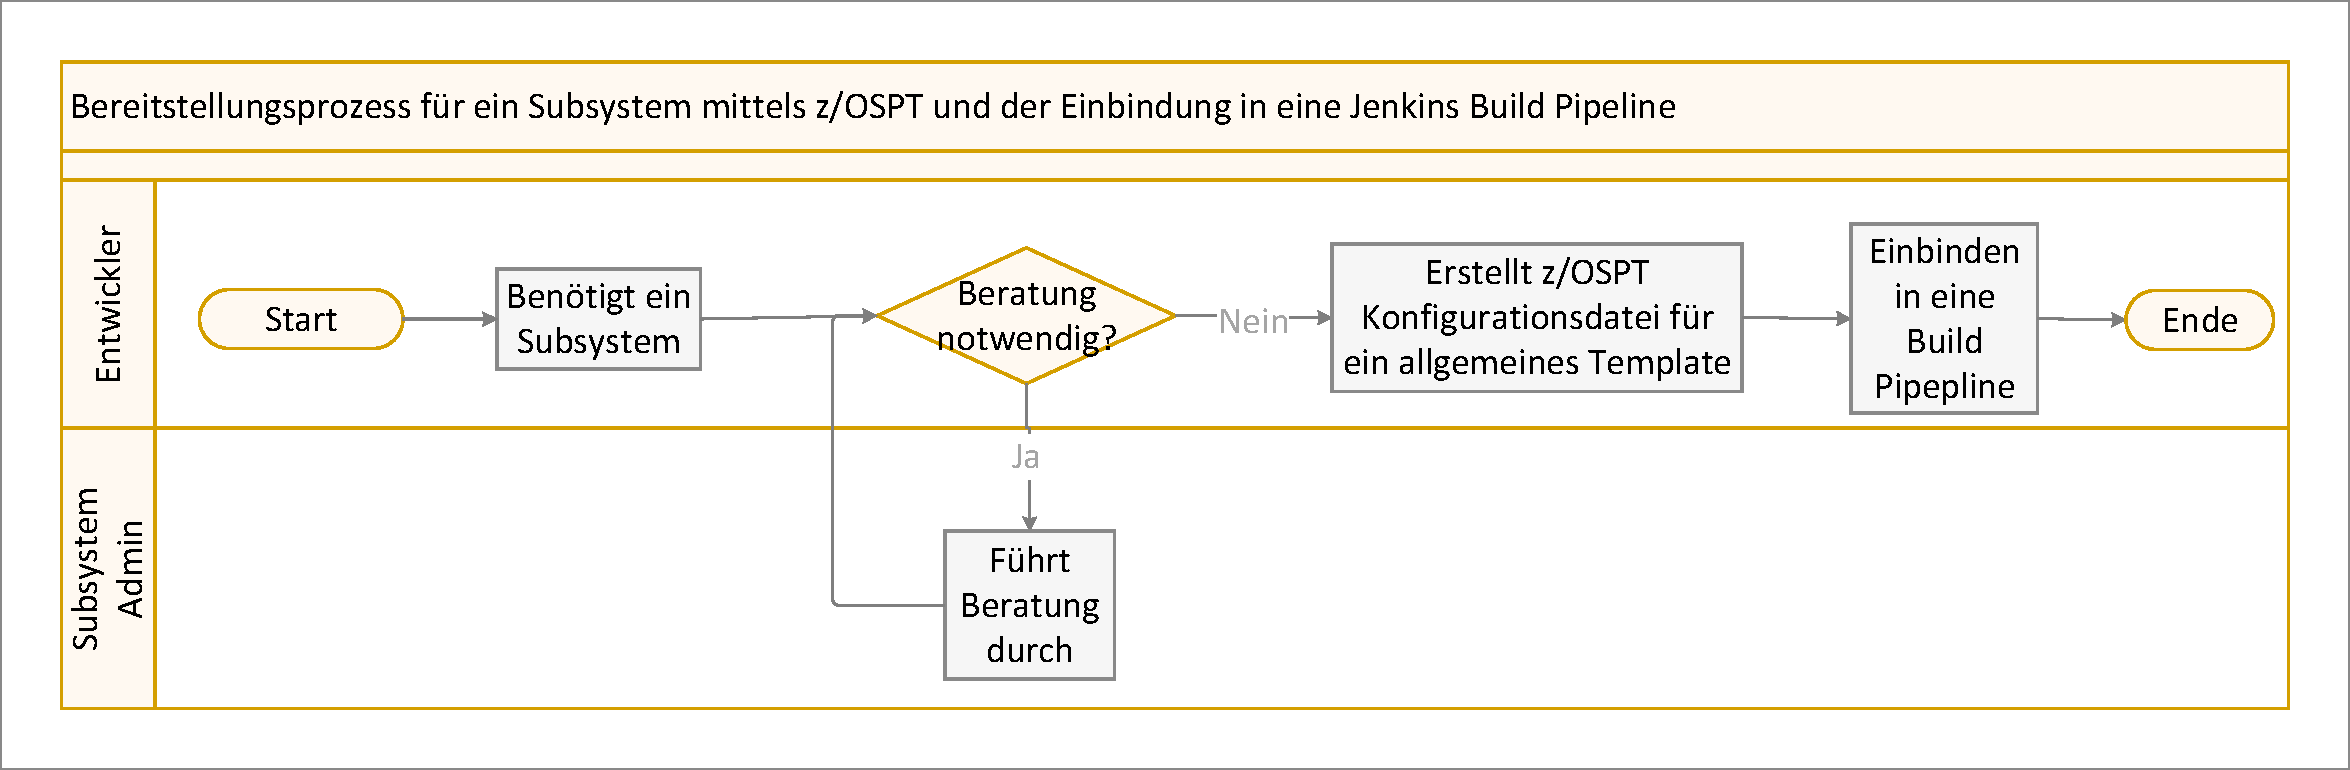
\includegraphics[width=\paperwidth,angle=90]{figures/swimlaneNeuerProzess.pdf}
\caption{Bereistellungsprozess eines Subsystems mittels einer z/OSPT Konfigurationsdatei}
\label{fig:proneu}
\end{figure}


